\PassOptionsToPackage{table}{xcolor}
\documentclass[sigconf]{acmart}
\usepackage{caption}
\usepackage[T1]{fontenc}
\usepackage[latin1]{inputenc}
\usepackage{subcaption}
\usepackage{todonotes}
\usepackage{graphicx}
\newcommand{\TODO}[1]{\todo[inline]{#1}}
\newcommand{\FILE}[1]{\todo[inline,color=green!20]{File: #1}}

\newcommand{\OK}{+}
\newcommand{\OP}{o}
\newcommand{\NA}{n/a}

\definecolor{lightgray}{gray}{0.94}
\let\oldtabular\tabular
\let\endoldtabular\endtabular
\renewenvironment{tabular}{\rowcolors{2}{lightgray}{white}\oldtabular}{\endoldtabular}

\setcopyright{none}
\copyrightyear{2022}
\acmYear{2022}
\acmDOI{}

\acmConference[White Paper]{White paper produced by the NIST Public Working Group on Big Data}{White paper produced by the NIST Public Working Group on Big Data}{Washington, D.C.}
\acmBooktitle{White paper produced by the NIST Public Working Group on Big Data, Washington, D.C.}
\acmPrice{}
\acmISBN{}
%%\citestyle{acmauthoryear}

\makeatletter
\def\@copyrightspace{\relax}
\makeatother

\begin{document}

\title{Reusable Hybrid and Multi-Cloud Analytics Service Framework}

\author{Gregor von Laszewski}
\email{laszewski@gmail.com}
\orcid{0000-0001-9558-179X}
\affiliation{%
  \institution{University of Virginia}
  \streetaddress{Biocomplexity Institute\\
                Town Center Four\\
                994 Research Park Boulevard}
  \city{Charlottesville}
  \state{VA}
  \postcode{22911}
  \country{USA}
}

\author{Wo Chang}
\email{wchang@nist.gov}
\affiliation{%
  \institution{NIST}
  \streetaddress{100 Bureau Drive}
  \city{Gaithersburg}
  \state{MD}
  \postcode{20899}
  \country{USA}
}

\author{Russell Reinsch}
\email{russell@mcleansystemsintegration}
% \orchid{idk}
\affiliation{%
  \institution{McLean Systems Integration}
  \streetaddress{6102 Franklin Park}
  \city{McLean}
  \state{VA}
  \postcode{22101}
  \country{USA}
}

\author{Geoffrey C. Fox}
\email{gcfexchange@gmail.com}
\affiliation{%
  \institution{University of Virginia}
  \streetaddress{Biocomplexity Institute\\
                Town Center Four\\
                994 Research Park Boulevard}
  \city{Charlottesville}
  \state{VA}
  \postcode{22911}
  \country{USA}
}

\author{Olivera Kotevska}
\email{kotevskao@ornl.gov}
%\orcid{0000-0001-9558-179X}
\affiliation{%
  \institution{Oak Ridge National Laboratory}
  \city{Oak Ridge}
  \state{TN}
  \postcode{37830}
  \country{USA}
}

\author{Ali ...}
\email{laszewski@gmail.com}
\orcid{0000-0001-9558-179X}
\affiliation{%
  \institution{University of Virginia}
  \streetaddress{Biocomplexity Institute\\
                Town Center Four\\
                994 Research Park Boulevard}
  \city{Charlottesville}
  \state{VA}
  \postcode{TBD}
  \country{USA}
}

\author{Gary ...}
\email{laszewski@gmail.com}
%\orcid{0000-0001-9558-179X}
\affiliation{%
  \institution{Oak Ridge National Laboratory}
  %\streetaddress{Biocomplexity Institute\\
  %              Town Center Four\\
  %              994 Research Park Boulevard}
  \city{Charlottesville}
  \state{VA}
  \postcode{TBD}
  \country{USA}
}


\author{PW ...}
\email{laszewski@gmail.com}
%\orcid{0000-0001-9558-179X}
\affiliation{%
  \institution{Oak Ridge National Laboratory}
  %\streetaddress{Biocomplexity Institute\\
  %              Town Center Four\\
  %              994 Research Park Boulevard}
  \city{Charlottesville}
  \state{VA}
  \country{USA}
}

\renewcommand{\shortauthors}{G. von Laszewski, et al.}

%% Whitepaper on Reusable Hybrid and Multi-Cloud Analytics Service Framework

% Gregor von Laszewski and Wo Chang and Russell Reinsch and Olivera
% Kotevska and Ali Karimi and Abdul Rahman Sattar and Garry Mazzaferro
% and Geoffrey C. Fox

\begin{abstract}

\FILE{section-abstract.tex}

Over the last several years, the computation landscape for conducting
data analytics has completely changed. While in the past, a lot of the
activities have been undertaken in isolation by companies, and
research institutions, today's infrastructure constitutes a wealth of
services offered by a variety of providers that offer opportunities
for reuse, and interactions while leveraging service collaboration,
and service cooperation.

This document focuses on expanding analytics services to develop a
framework for reusable hybrid multi-service data analytics. It
includes (a) a short technology review that explicitly targets the
intersection of hybrid multi-provider analytics services, (b) a small
motivation based on use cases we looked at, (c) enhancing the concepts
of services to showcase how hybrid, as well as multi-provider services
can be integrated and reused via the proposed framework, (d) address
analytics service composition, and (e) integrate container
technologies to achieve state-of-the-art analytics service deployment
capabilities.

\end{abstract}


\begin{CCSXML}
<ccs2012>
   <concept>
       <concept_id>10002951.10003227.10003241.10003244</concept_id>
       <concept_desc>Information systems~Data analytics</concept_desc>
       <concept_significance>500</concept_significance>
       </concept>
   <concept>
       <concept_id>10010520.10010521.10010537.10003100</concept_id>
       <concept_desc>Computer systems organization~Cloud computing</concept_desc>
       <concept_significance>500</concept_significance>
       </concept>
   <concept>
       <concept_id>10011007.10011006.10011072</concept_id>
       <concept_desc>Software and its engineering~Software libraries and repositories</concept_desc>
       <concept_significance>500</concept_significance>
       </concept>
 </ccs2012>
\end{CCSXML}

\ccsdesc[500]{Information systems~Data analytics}
\ccsdesc[500]{Computer systems organization~Cloud computing}
\ccsdesc[500]{Software and its engineering~Software libraries and repositories}


\keywords{Analytics, hybrid cloud analytics services, heterogeneous cloud analytics services, service catalog}

\FILE{section-abstract.tex}

\begin{abstract}
    
This document summarizes the NIST Analytics Service
Framework that targets to analytics functionalities to be hosted on
computational resources including Clouds, Containers, and High
Performance Computing (HPC). Although we use the REpresentational
State Transfer (REST) to formulate some details of the architecture,
it is independent from REST and can be formulated in other
frameworks. While using REST we use a familiar pattern for architect,
implementer, and strategists. Due to the many frameworks, programming
languages and services supporting REST the architecture can easily be
enhanced and implemented with various technical solutions.  The
analytics framework also targets big data. Big data is a term used to
describe extensive datasets, primarily in the characteristics of
volume, variety, velocity, and veracity. While opportunities exist
with Big Data analytics, the data characteristics can overwhelm
traditional technical approaches, and the growth of data is outpacing
scientific and technological advances in data analytics. To advance
progress in Big Data analytics, the NIST Big Data Public Working Group
(NBD-PWG) is working to develop consensus on important fundamental
concepts related to Big Data. The results are reported in the NIST Big
Data Interoperability Framework (NBDIF) series of volumes.

\end{abstract}

\maketitle

%%%%% \FILE{section-production.tex}

\section*{Report Production}


This document is conducted as part of the NIST \WG. The working group
holds public meetings regularly Tuesdays at 1 pm. The
working group is public, and anyone can join that is interested in
contributing to this document and bringing it to completion. We will
be using GitHub to coordinate this work. Although the work is done in
a public working group, we had one member of the group asking to keep
the document private. As such, you need to join our meeting group first
before we grant you access to this document. You can join the working
group by contacting Wo Chang at \verb|wchang@nist.gov|.


The production of this document is conducted to address the following
needs

\begin{enumerate}
  \item a one-page executive summary, 

  \item a detailed specification,

  \item use cases that support this document that may be hosted in
    separate documents. Such documents could follow the template as
    provided at \cite{nist-bigdatawg}.

\end{enumerate}


\parindent0pt We are using the following tools to manage the completion of
the document:

\begin{itemize}

\item
  \href{https://www.overleaf.com/project/619ba513e4aade4400e06df8}{an
    online document $\rightarrow$} we work on in Overleaf,

\item \href{https://github.com/orgs/cyberaide/projects/1}{a task list
  $\rightarrow$} in GitHub,

\item \href{https://github.com/orgs/cyberaide/}{a versioned document
  source $\rightarrow$} in GitHub,

\item \href{https://nist-analytics.slack.com}{a slack channel
  $\rightarrow$} to increas the communication outside of the Working
  group meetings and to coordinate task.

\end{itemize}

Once you have joined the Working group, you can get access to the
document directories by contacting \url{laszewski@gmail.com}.

\begin{quote}

{\em Please note that we stopped using Word for the document
  management contributors consistently used different templates and
  formatting rules resulting in unsustainable multi hourlong cleanups
  every week instead of being able to focus on content. For this
  reason, we will not switch back to Word. However, a section could be
  written in markdown, which can easily be integrated into the
  document. Formatting should be kept at a minimum.}

\end{quote}




\FILE{section-summary}

\section{Introduction}
\label{sec:summary}


Analytics as a service has become a multi-billion dollar opportunity
for the industry. Companies and research institutions offer a number
of competing but also collaborating services. While in the past
emphasize was placed on the hybrid multi-cloud infrastructures, the
focus is significantly shifting to offering {\em analytics services}
and not just infrastructure to customers and researchers. As such, it
is important to identify how researchers can interoperate with
services offered by various service providers. Analog to the
terminology in cloud computing, we introduce the terms {\em hybrid}
analytics services that include services run by remote service
providers or by the organization on local resources. In addition, we
use the term {\em multi} analytics services to indicate that multiple
services from potentially multiple service providers work in concert
to offer a new capability released to users as analytics
services. While applying such services to data, we term the
combination of such services as {\em hybrid multi-services data
  analytics} services. If properly put in place, the resulting service
accelerates new solutions offered by industry and research as new
services with a combined new functionality.

To achieve this, it does require a level of platform-independent
interoperability.  To assure that the pathway to
leverage these hybrid and multi-analytics services is kept at a high level
while at the same time exposing enough details, we need to support
intelligent decision-making as part of the service
orchestration. Services must be chosen to fulfill a set of {\em
  analytics service} level requirements posed by the users. It is of particular
interest how we can formulate hybrid analytics services and
multi-analytics services offered by different providers that provide
other features. The user needs to specify this via a simple analytics
service provider independent specification.

Our data analysis intends to be able to determine which service is
suitable or chosen based on its requirements and to what degree
reusability is offered while replicating the analysis across different
services. Hence we will work towards a {\em ``Reusable Hybrid
Multi-Services Data Analytics Framework''}. This results in a research
platform that allows the creation of of integrated application
platform benefitting fromreusable hybrid analytics services.


By integrating such services, we will be able to significantly impact
data analytics while leveraging not only one vendor's implementation
but by promoting the reuse services via a {\em many-vendors}
approach. Not only that, but we will also allow the interplay between
different approaches while offering a uniform specification platform.
Because we target the topic of this interplay, the effort has been
done in collaboration with the NIST Information Access Division (IAD).

The paper is structured as follows. First we present initially the
motivation leading up to this work (Section~\ref{s:background}),
followed by a discussion about Reuirments that we derived by analysing
a number of complex usecases. Next we present our architectural
approach, which is based on lessons learned from the reuirements we
have gathered and lessons learned during our implementation
(Section~\ref{s:arch}. We present an architectural design capable of
supporting the needs we have identified.  Finally, we present our
conclusions (Section~\ref{sec:conlcusion}).


\FILE{section-background.tex}



find parameter for single case

now we have services

now how do we deploy this to many millions - use registry to implement that




\section{Motivation}\label{s:background}

In this section, we explain the motivation  while summarizing
briefly, the different concepts constituting our work.

\subsection{Hybrid Analytics Services}

A {\em hybrid analytics service} combines the strength of analytics
services that are offered by providers in public, private, or
on-premise. It leverages them in order to provide ideally optimized
orchestration across them. This is not just limited to reducing cost,
but also to address security and privacy concerns when the data
analytics or the data to perform the analytics can not be hosted in
public clouds. Many of the major cloud providers such as AWS, Azure,
Google, IBM, Oracle, and others have made hybrid clouds a cornerstone
of their business model, with each of them mainly pushing their own
solutions. Recently, however, we see that the focus is no longer
offering just infrastructure but instead to provide services hiding the
cloud infrastructure entirely from the users.  This leads to vendors
also start providing hybrid analytics solutions that may integrate
multiple services offered by various providers resulting in solutions
with heterogenous service offerings. The integration of such services
provides challanges as each vendor may conform to different
integration solutions adressing public, private and on-premise
analytics services. In general, customers will benefit from a more
integrated approach to ease deployment and management concerns.

\subsection{Multi-Analytics Services}

Over the last two years, we have seen an explosion of analytics
services, mainly through the integration of AI and deep learning
services. High-level analytics services are being developed that hide the
complex infrastructure needed to embed not only services from one
vendor but multiple vendors. Hence we speak of {\em multi-analytics
  services}. These services can then be used in cooperation or
competition. We cooperate if services enhance each other, we compete
if a service is chosen over another service due to better service
level agreements. Through this interplay of the services, it is
beneficial to formalize this interoperability. In the case of competition,
we also need to be able to formulate a competing service that then
calls out other services to implement the desired analytics task.

\subsection{Enhancing the Big Data Reference Architecture}
\label{s:arch}

NIST has developed a Big Data Reference Architecture as part of
NBDIF\cite{nist-v6} and identified a number of use cases that motivate
it \cite{nist-v3}. We can leverage the effort
~\cite{nist-v1,nist-v2,nist-v3,nist-v4,nist-v5,nist-v6,nist-v7,nist-v8,nist-v9}
while formulating novel interoperability specifications that arise in
our effort that has not been addressed. While we previously focused
mostly on virtual machine management, this effort will enhance the
activities to include high-level coordinated service deployments and
utilization while leveraging containers.

\subsection{Identification of State-of-the-Art Data Analytics Patterns}

We have to ask why this opportunity can be addressed now to enable
this interplay?  It is clearly motivated by state-of-the-art data
analytics capabilities that only recently have become available.
Although government agencies have provided some of the most capable
high-end computing systems over the last years, they have integrated
specialized GPUs as well as container technologies to bring forward
new data analytics capabilities in these on-premise services. Industry
has provided advanced analysis capabilities for some time but only
recently they have achieved the maturity allowing reuse and
cooperation opportunities among all of them.

We like to provide a scenario that motivates our work. A health care
technician in the hospital uses voice commands to control an MRI
machine to take tomographic images. The images will be automatically
sent to a private analytics service to identify if the images contain
signs of COVID-19. Not only is one service consulted, but multiple to
assure that the best available algorithms are chosen. Once identified,
the image sare sent to a public analytics service (if the patient consents) in
order to improve the available images to improve the deep learning data
analysis. Previous images that have tested negative may be reanalyzed
with the newly improved models. If new cases are found based on
the improved analysis, health care providers are notified, and further
actions regarding the treatment plan by the supervising physician is
cast. As we can see, this example has all the ingredients that we need
to create a new generation of services that integrates on-premise
infrastructure, public and private services. The orchestration of the
services as well as a convenient interface. Automation of the workflow
of this use case example is explicitly stated.

Analyzing this example, we identify a mixture of services that utilize
on-premise infrastructure (the MRI), private and public services. A
variety of service patterns are used in concert to establish an analysis
pipeline targeted explicitly for this application use case. 

The goal of this work is to analyze the interoperability of such
service scenarios and identify such patterns motivating a vendor
neutral architecture that promotes reusable implementations to 
support aspects of similar use cases addressed by them.


\FILE{section-introduction.tex}

\newcommand{\WG}{\TODO{Wo: define name of wrking group}{WORKINGGROUP}}

\section{Introduction}


\subsection{Background}



\subsection{Scope and Objectives}

NBD-PWG\footnote{\TODO{introduce in the background section. THe
background section has been integrated here. check valitity and fix
somehow.}} is exploring how to extend
NBDIF \footnote{\TODO{introduce in the background section. THe
background section has been integrated here. check valitity and fix
somehow.}} for packaging scalable analytics as services to meet the
challenges of today's information analytics. These services are
intended to be reusable, deployable, and operational for Big Data,
High Performance Computing, AI machine learning (ML), and deep
learning (DL) applications, regardless of the underlying computing
environment.

This document explores key focus areas and document level of interest
from industry, government, and academia in extending the NBDIF to
develop scalable analytics as services that are reusable, deployable,
and operational, regardless of the underlying computing environment.
\TODO{Russel: note that the 'string' reusable, deployable, and
  operational was also used in the previous ppg.}


The work has been conducted with input from the NIST BIg Data Working
group while enhancing their original activities to address
requirements for Analytics Service. This includes hosted on
computational resources including Clouds, Containers, and High
Performance Computing (HPC), thus targeting analytics services hosted
on premis, private and public clouds. We have chosen REpresentational
State Transfer (REST) to formulate some details of the architecture,
it is independent from REST and can be formulated in other
frameworks. While using REST we use a familiar pattern for architect,
implementer, and strategists. Due to the many frameworks, programming
languages and services supporting REST the architecture can easily be
enhanced and implemented with various technical solutions.


TBD:

The
analytics framework also targets big data.
Big data is a term used to
describe extensive datasets, primarily in the characteristics of
volume, variety, velocity, and veracity. While opportunities exist
with Big Data analytics, the data characteristics can overwhelm
traditional technical approaches, and the growth of data is outpacing
scientific and technological advances in data analytics.

To advance
progress in Big Data analytics, the NIST Big Data Public Working Group
(NBD-PWG) is working to develop consensus on important fundamental
concepts related to Big Data. The results are reported in the NIST Big
Data Interoperability Framework (NBDIF) series of volumes.



\FILE{section-definitions.tex}

\section{Definitions and Concepts}
\label{sec:definitions}

In this section we provide a list of definitions and doncepts that
help communication between different interdisciplinary groups while
allowing them to use the same language.

\begin{description}

\item [NBD-PWG] TBD

\item[NBDIF] TBD

\end{description}



\FILE{section-usecases.tex}

\section{Use Cases for Analytics Services}
\label{sec:usecases}


\subsection{Use Case Development Process}

To specify use cases for our analytics framework, we encourage contributors to contact us and provide us with their high-level descriptions of their use cases. The use cases should be focusing on highlighting one or multiple aspects of the features related to analytics frameworks. While inspecting the various features we intend to collect and analyze them in various contexts that are relevant for analytics users. The lessons learned from this analysis are to be integrated into this document in order to formulate a comprehensive vendor neutral analytics framework.
Use cases can be formulated in various format but should include diagrams that make them easy to comprehend as well as allowing the reader to extract the specific analytical aspects. Such diagrams can include functional cross diagrams, process diagrams and others.
Use cases should especially address the use of metadata describing the functional and the data related properties. This includes metadata related to time, space, exchange/protocols, privacy, and security related aspects.
A functional description of the use case is to be included as a subsection called Functionalities and Activities. This section is mirroring our experience with documenting use cases as part of the Big Data Application Provider of NBDIF Reference Architecture. Hence, we assume the following draft form for a use case:

\begin{description}
\item[Title:] 		Title of the use case
\item[Contributor:] 	The list co contributors
\item[Description:] 	One to two sentences about major functionalities and activities with respect to the sample cross-functional diagram
	
	\begin{description}
	\item[Cross-Functional Diagram:]
		Inclusion of a cross functional Diagram, alternatively other diagrams could be 			chosen.
	\item[Functionality Activities:]
	\begin{enumerate}
        \item Activity \#1 – description…
        \item ...
        \item Activity \#n – description…
    	\item Use Case Summaries
    \end{enumerate}
\end{description}
\end{description}

\begin{figure}[htb]
    \centering
    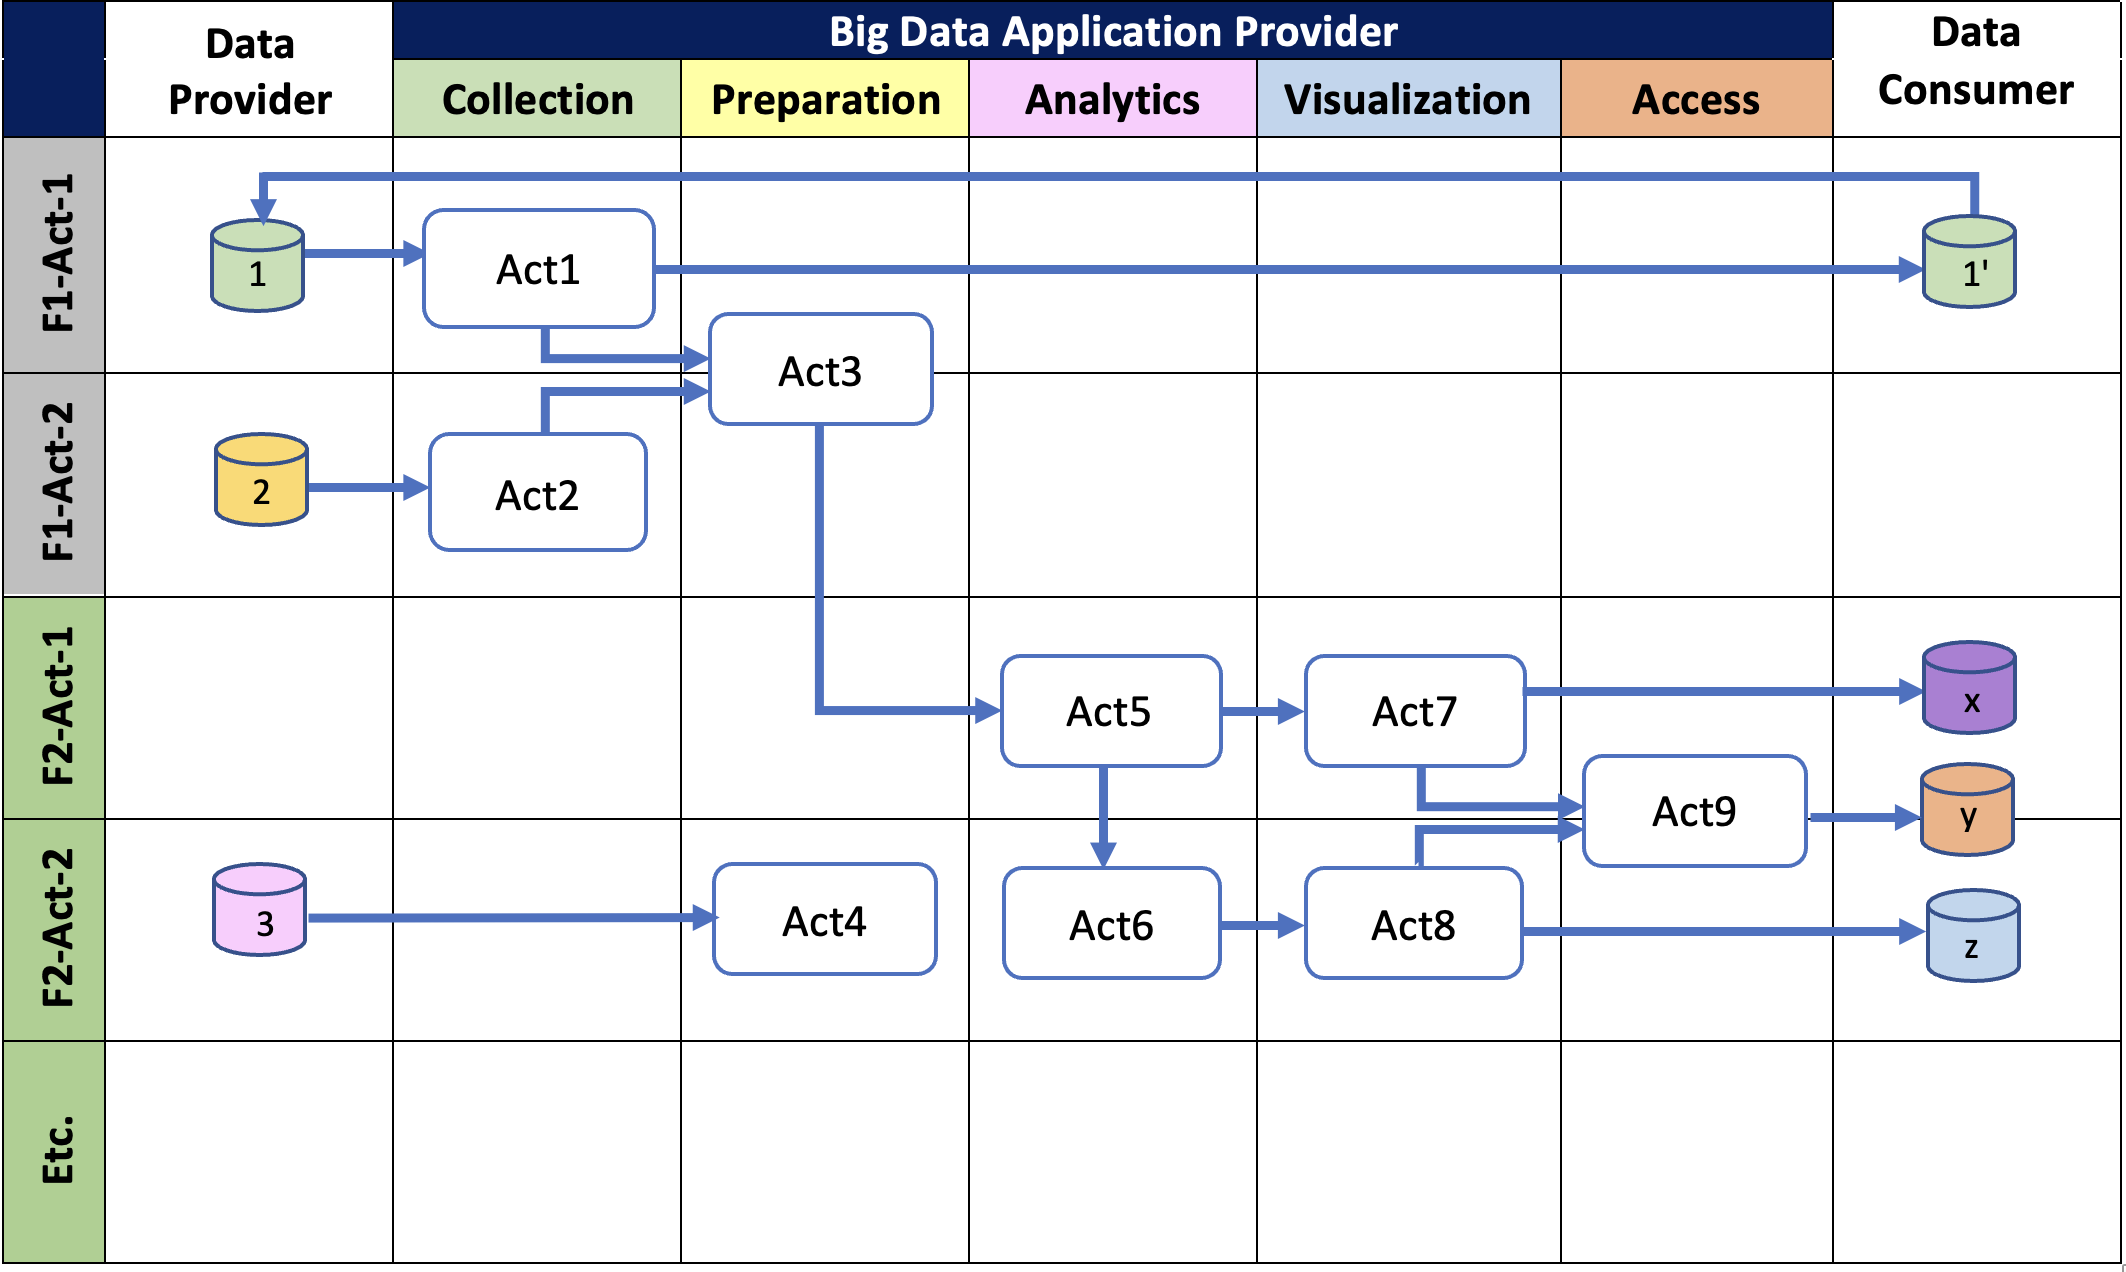
\includegraphics[width=1.0\columnwidth]{images/cross-functional-diagram.png}
    \caption{Cross-functional Diagram}
    \label{fig:cross-functional-diagram}
\end{figure}


Next, we will list use case summaries and if available point to specific publications on the NBDIF Web page that include more details. The expectation of this section is to
 
\begin{itemize}
\item	Provide an overview of use cases that motivate this document
\item	It will summarize requirements that we obtain from these use cases that influence how we proceed.
\end{itemize}

As a result, we identify how they fit into the workflow of data analytics. This includes the description of a subset of functionality that is used in general by data analytics.  In particular, it described the relationship between input and output of data analytics components and interfaces.  The use case summaries are expected to be available through the BigDataWG Web page and includes currently the following examples:

\begin{enumerate}
\item	\href{https://bigdatawg.nist.gov/_uploadfiles/M0701_v1_2020102001.docx}{M0701} – Use case template \cite{nist-usecase-template}
\item	\href{https://bigdatawg.nist.gov/_uploadfiles/M0702_v1_2020102002.pdf}{M0702} - Numeric weather prediction \cite{nist-wrf}
\item	\href{https://bigdatawg.nist.gov/_uploadfiles/M0703_v1_2020102003.pdf}{M0703} - HVAC Heat ventilation and air conditioning \cite{nist-hvac}
\end{enumerate}



\FILE{usecase/weather.tex}
\subsection{Use Case: Numeric Weather Prediction}

\paragraph*{Background.} Large amounts of weather data ar e produced continually and stored in
many different databases.  Accurate weather predictions require large
amount s of processing power to accurately simulate conditions
worldwide at a high resolution and fre quent intervals. One of the
most computationally consuming parts of a reliable weather model is th
e microphysics scheme. The current microphysics scheme, Weather
Research and Forecasting (WRF) Single Moment 6-class Microphysics
(WSM6), simulates the processes in the atmosphere that leadto the
formation and precipitation of rain, snow, and graupel and requires
complex floating-point operations needing to be performed on vast
amounts of data for accurate simulations. As computer
performanceimproves, so does the Numerical Weather Prediction (NWP)
models' resolution and accuracy. However, there is still much progress
to be made, as simulation accuracy still falls off sign ificantly for
predictions more than 36 hours in advance. Figure \ref{fig:weather-1}
shows the general WRF modeling system flow chat.

\begin{figure}[htb]
\centering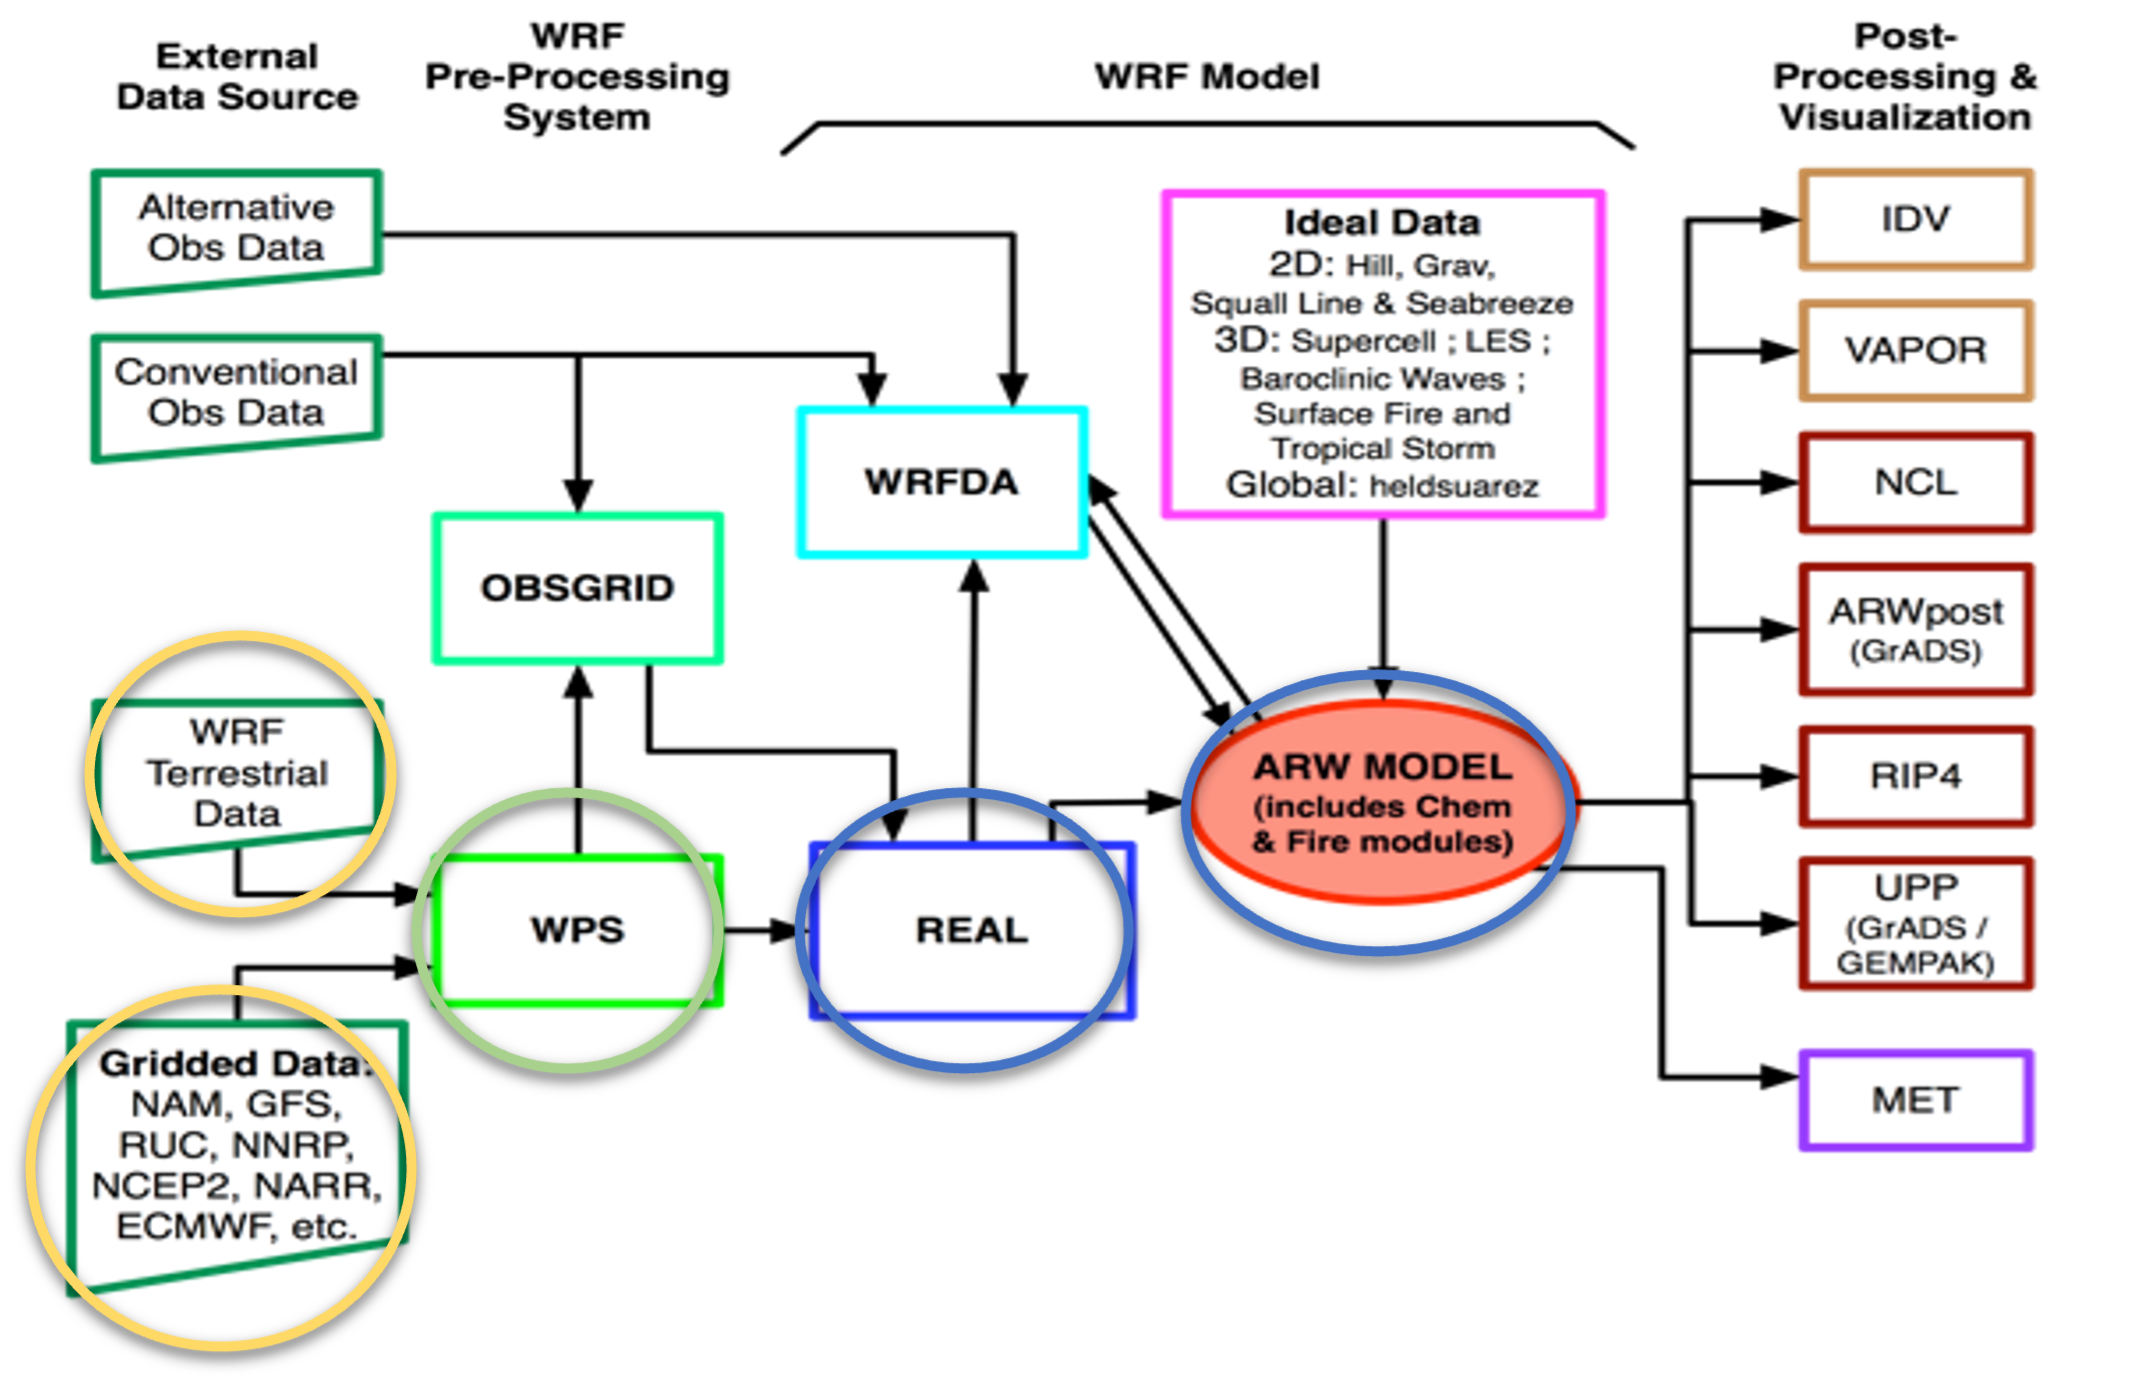
\includegraphics[width=1.0\columnwidth]{usecase/nwp-arch.png}
\label{fig:weather-1}
\caption{WRF Modeling System Flow Chart with Various Configuration.} 
\end{figure}

\paragraph*{Functionalities and Activities} (based on Big Data Application Provider of NBDIF Ref. Architecture).
In this case study, we only focus on two main functionalities, namely
WPS and WRF, and their activities.  Figure \ref{fig:weather-2} shows
the cross-functional diagram for their actions.

WPS Activities:

\begin{figure}[htb]
\centering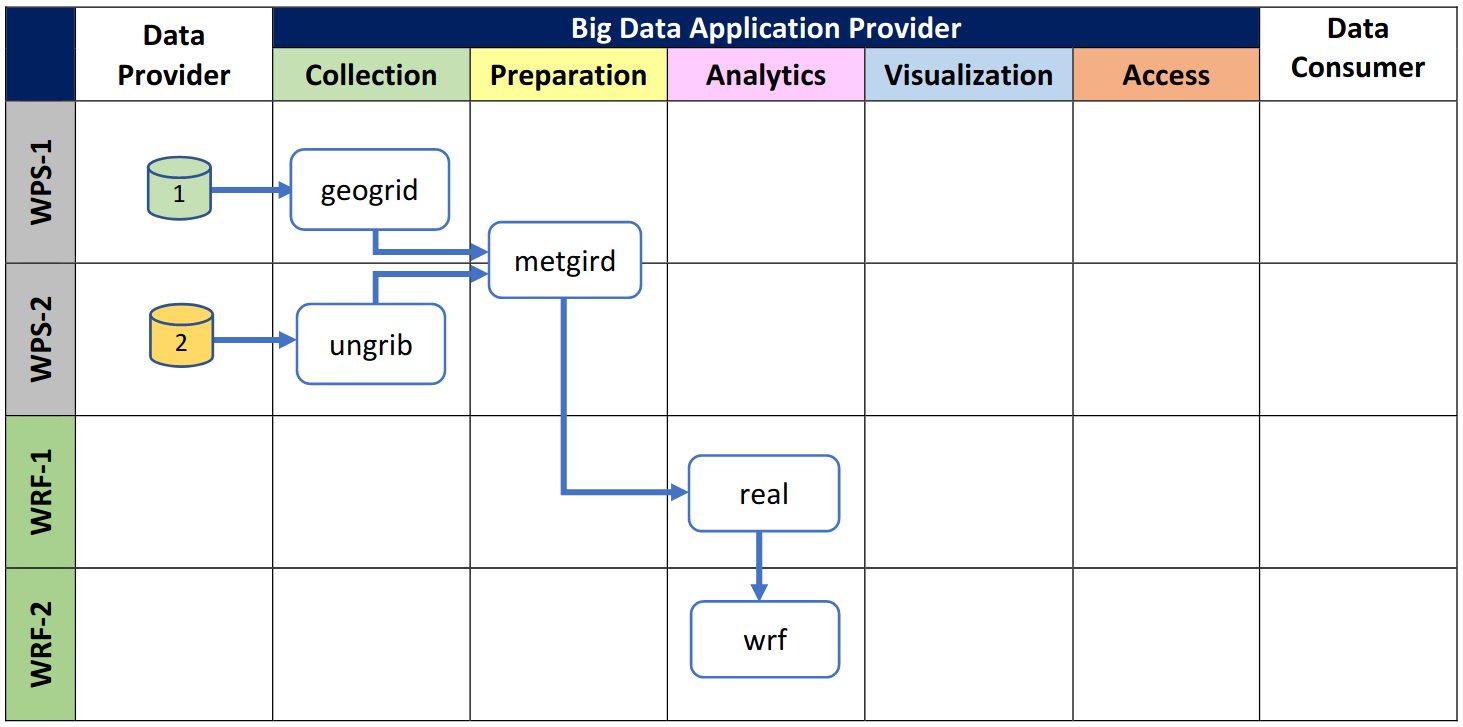
\includegraphics[width=1.0\columnwidth]{usecase/weather.png}
\label{fig:weather-2}
\caption{Cross-Functional Diagram Numerical Weather Prediction.}
\end{figure}

\begin{enumerate}
  
\item geogrid -- defines simulation domains and interpolate various terrestrial data sets to the
model grids. Input data available at [1].

\item ungrib -- extracts needed meteorological data and packs it into an intermediate file format.
Input data available at [2]

\item medgrid -- prepares horizontally interpolate the meteorological data onto the model domain.
  Input data from the output of geogrid and ungrib.

\end{enumerate}

WRF Activities:

\begin{enumerate}

\item real -- prepares vertically interpolates the output from metgrid, and creates a boundary and initial
condition files with some consistency checks.

\item wrf -- generates a model forecast.

\end{enumerate}

\paragraph*{Datasets.}

\begin{enumerate}
  
\item WRF Users Page, WPS V4 Geographical Static Data Downloads Page \cite{wrf-data}

\item NCEP FNL Operational Model Global Tropospheric Analyses, continuing
from July 1999 \cite{cisl_rda_ds083.2}

\end{enumerate}

\FILE{usecase/hvac.tex}
\subsection{Use Case: HVAC Recommendation}

\TODO{??}{move to authors: Olivera Kotevska, Research Scientist, Oak Ridge National Laboratory, U.S.A.}

\paragraph*{Background.}

Continuous streaming data is produced by heat ventilation and air conditioning (HVAC) systems every
day from the residential houses. This data is stored in a databased on the cloud as it arrives. The data
is used to calculate what should be the next HVAC set point in the house with respect to user
preferences. Periodic recommendations considering environmental parameters, user comfort level
and past user preferences require advanced machine learning algorithm called reinforcement
learning [this sentence needs grammar edit]. Accurate recommendations can save energy and reduce cost. This functionality has three
parts Environmental Forecasting (EF), Learning from the past, (LP), and Set-Point Recommendation
(SPR). EF calculates weather temperature and price predictions. LP learns from the behavior in the
past. SPR model calculates next set-point based on past experience and EF predictions. Figure \ref{fig:hvac-1} shows
the general modeling system flow chat.

\begin{figure}[htb]
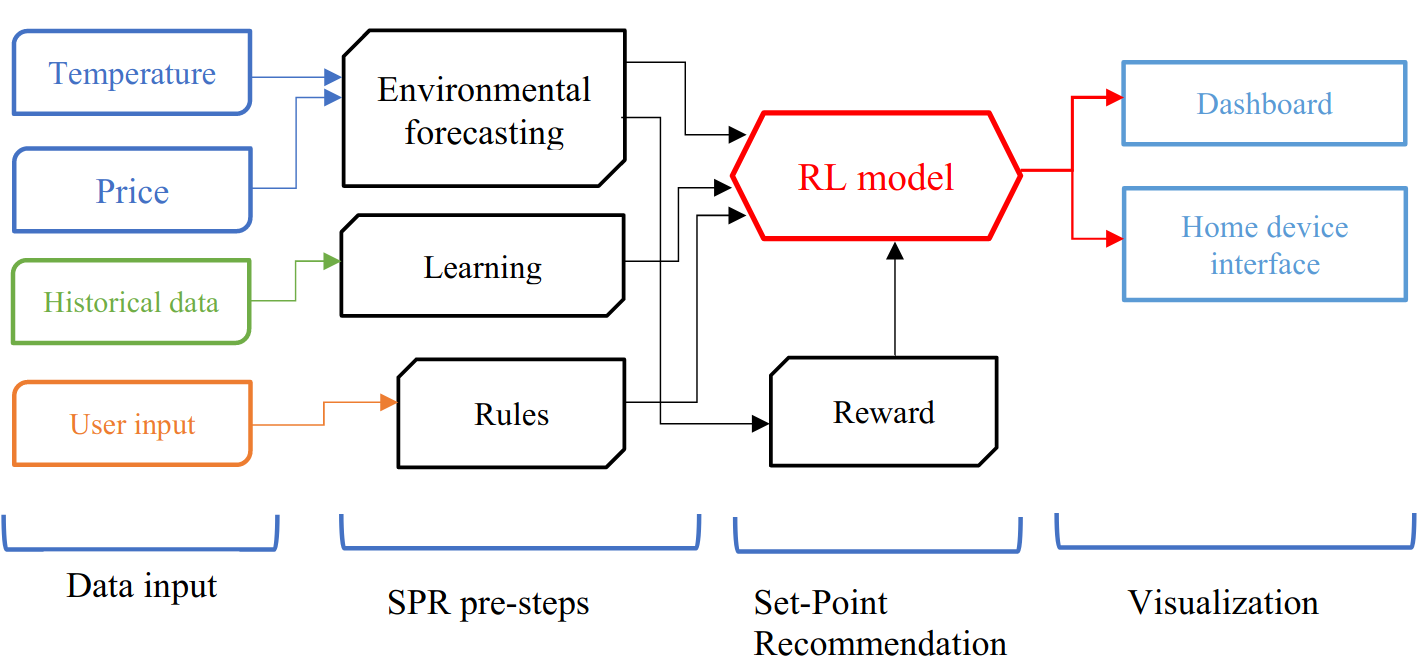
\includegraphics[width=1.0\textwidth]{usecase/hvac.png}
\label{fig:hvac-1}
\caption{HVAC general modeling system flow chat.}
\end{figure}


\paragraph*{Functionalities and Activities} (based on Big Data Application Provider of NBDIF Ref. Architecture).


In this case study, we only focus on three main functionalities, namely EF, LP and SPR, and their
activities. Figure \ref{fig:hvac-2} shows the cross-functional diagram for their actions.



\begin{figure}[htb]
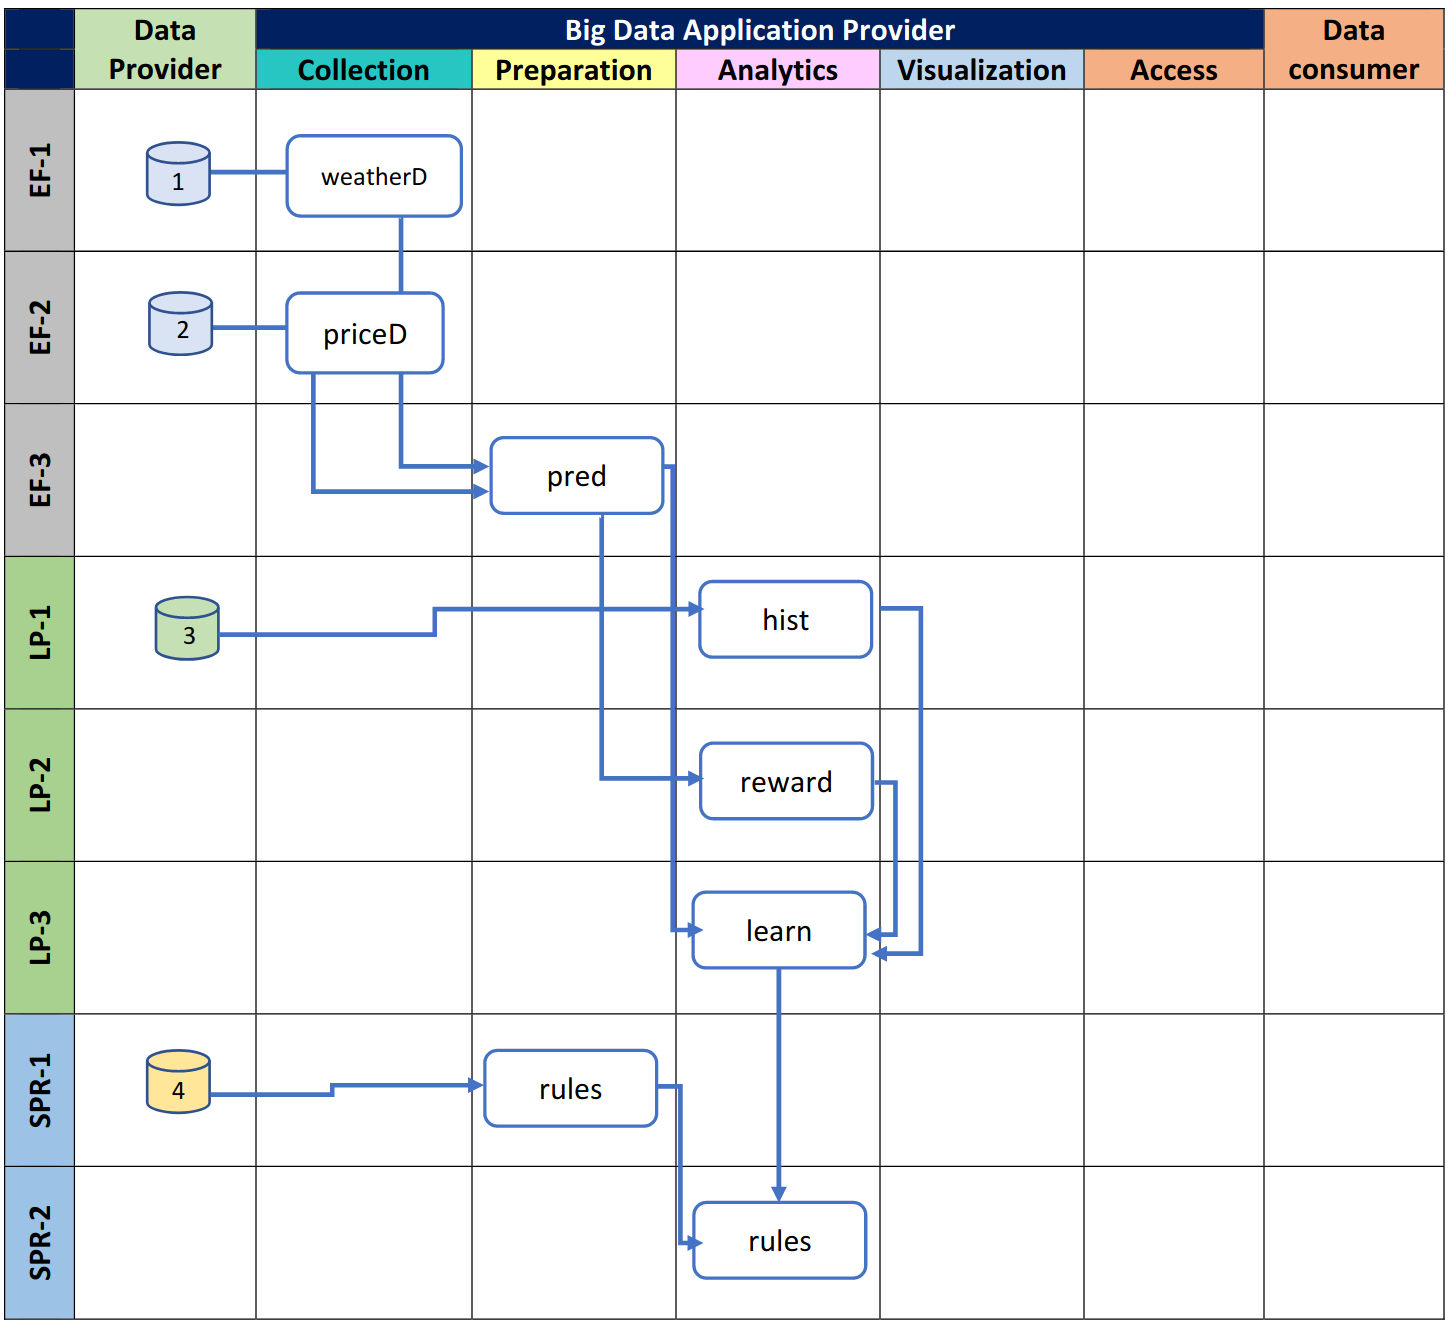
\includegraphics[width=1.0\textwidth]{usecase/hvac-2.png}
\label{fig:hvac-2}
\caption{Cross-Functional Diagram HVAC Recommendation.}
\end{figure}


EF Activities:

\begin{enumerate}
\item weatherD – Collects current weather temperature and predicted temperature for timestamp
X.
\item priceD – Collects current electricity price and predicted price for timestamp X.
\item pred – Extract needed data fields and packs it into an intermediate file format. Input data
from the output of weatherD and priceD.
\end{enumerate}


LP Activities:

\begin{enumerate}
\item hist – Prepares history data points and creates initial condition weights.
\item reward – Generates reward based on the current weatherD and priceD.
\item learn – Collects data from current weatherD, priced, reward.
\end{enumerate}

SPR Activities:

\begin{enumerate}
\item rules – Creates rules based on user preferences and conversion preferences.
\item rlmodel – Interpolates the output from learn, rules and generates set point recommendation
\end{enumerate}

\TODO{??}{No datasets provided.}



\subsection{Architecture}

To support our goal to enable the use of hybrid and multi-analytics
services, we will explore architectural patterns
that are conducive to use cases such as the one we outlined
previously. These patterns will be of general use as they can
be applied to other use cases. In our case, we will work towards an
architecture as depicted in Figure~\ref{fig:arch}.

\begin{figure}[htb]
  \begin{center}
    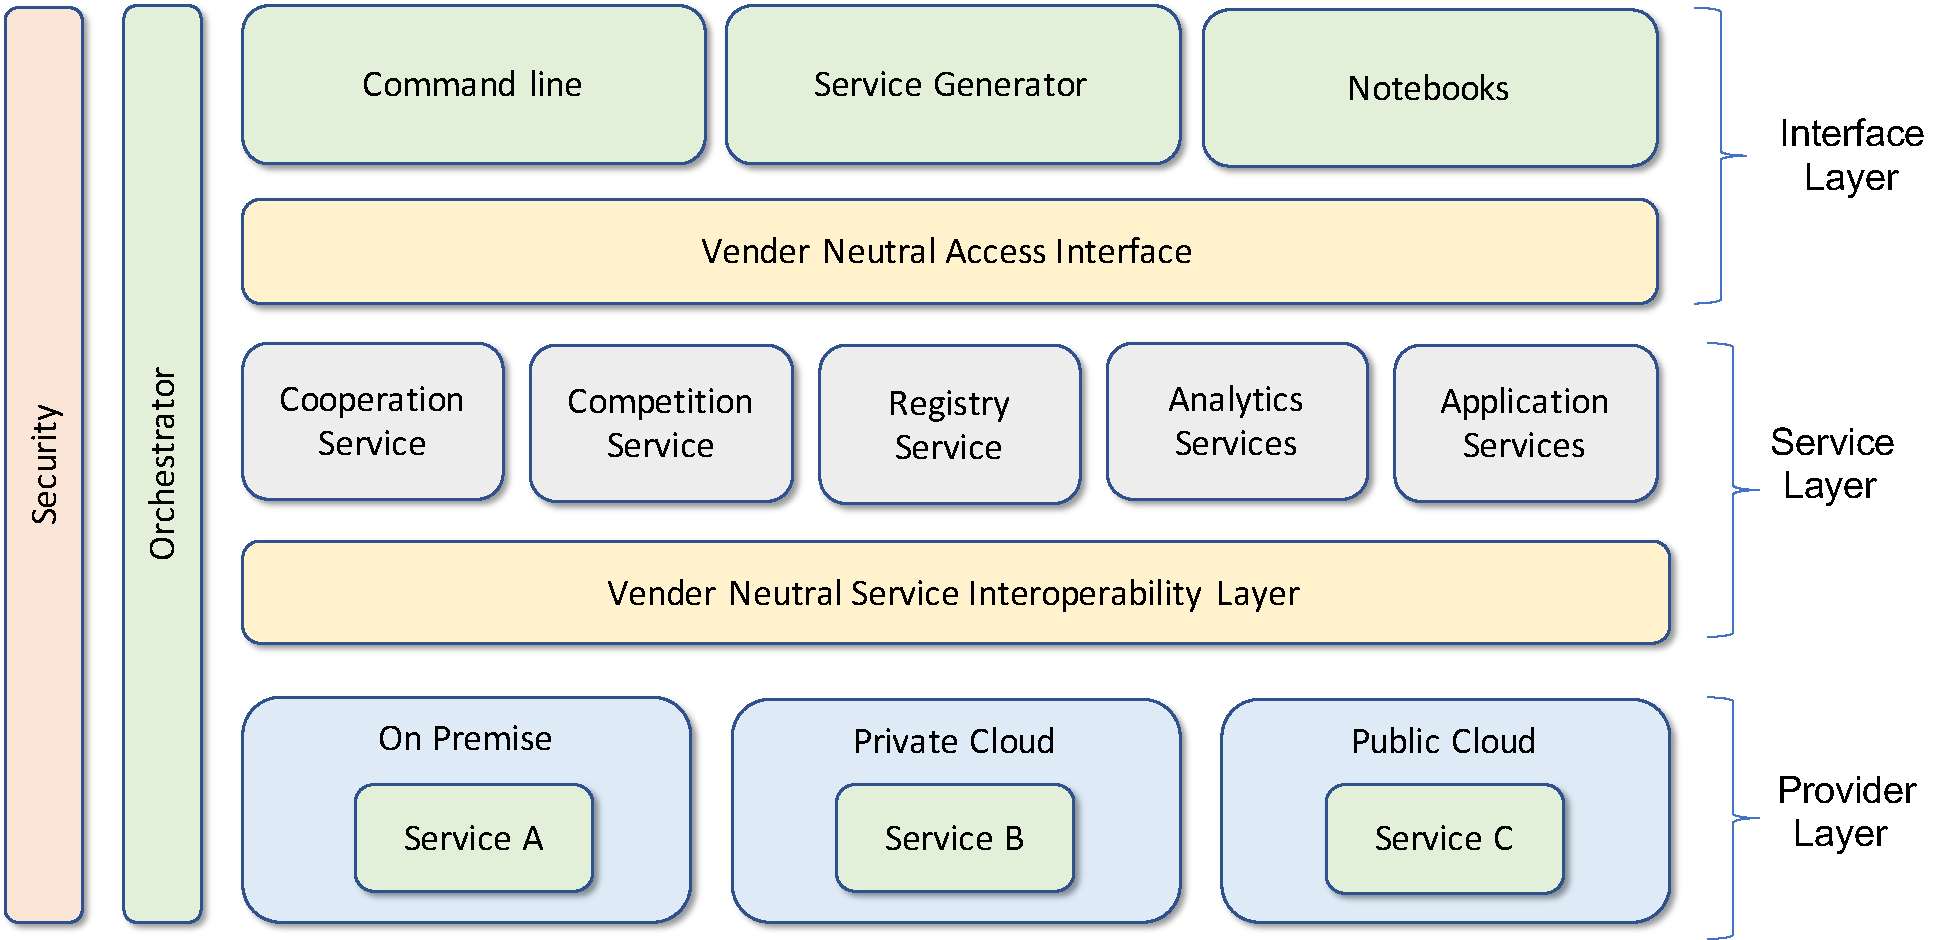
\includegraphics[width=1.0\columnwidth]{images/hybrid-service-arch.pdf}
    \end{center}
  \caption {Architecture of the hybrid multi-analytics service
    framework}
  \label{fig:arch}
\end{figure}

The architecture is organized as a layered architecture and contains
multiple components in each layer. We distinguish the interface,
service, and provider layer. Security and an orchestration service
enable the integration of the various components into a coordinated
application pipeline.

\subsection{Interface Layer}

Today’s analytics is invoked through a multitude of interfaces, making
it possible to invoke them in different languages, but also high level
frameworks. This is often achieved by an interface layer using REST
to communicate with the other layers. For our work, we will focus on
the command line interface promoting reuse in shells, Jupyter notebooks
showcasing the reuse in an interactive analysis capable framework, and
our previous work to generate REST services (see Section \ref{s:gas}).

\subsubsection{Command Line Interface}

To provide reusability within the DevOps application of data analytics
pipelines, we will provide an enhanced command-line interface that
specifically targets hybrid and multi-analytics environments. This is
facilitated by adding command options, shell variables, and
configuration files that can be passed into the commands.
Most importantly, we will be analyzing which specific parameters we
need to make available when investigating cooperative and competitive
services. The parameters can be directly translated to REST service invocations.

\subsubsection{Interactive Notebooks}

Although it is important to provide a command-line interface that can
easily be used to generate computing activities for solving data
analytics tasks, it is even more important that the framework can be
integrated into interactive steering tasks conducted directly by the
data scientists. For this, we leverage Jupyter notebooks and integrate
service calls to the backend system into the notebooks just as we can
in regular python programs. The difference here is that Jupyter
provides a rich set of interactive components and widgets that can be
leveraged to prototype interactive services but also parameter
studies. We will provide such notebooks as examples. While our
previous work has been integrated into notebooks, the capabilities of
notebooks were not yet fully utilized as the integration was done on
the service level but not on a level where Jupyter was used to enhance
the service pipeline. We will showcase full integration.

\subsection {Service Layer}

\subsubsection{Generalized Analytics Services}
\label{s:gas}

While we have focussed previously on the automated generation of
services using REST, we need to consider the other aspects of this
architecture that is needed to support the data analyst.  We have
shown that it is possible to create rest services from Python
functions and classes while augmenting them with helper services such
as data uploads. The development of such services is out of the
capability of many data scientists as they focus on developing
transformative data analysis functions and not on the infrastructure
service generation. Our work is lowering the bar for such
implementation and allowing even data analysts to generate reusable
REST services \cite{las21openapi}. The effort to learn about how to
create vendor-independent and computer language-independent services
has been reduced from months to days. We can leverage this effort to
generate application-specific services quickly. The services generated
are integrated into a user-managed service registry. We will leverage
this service and explore if Flask and FastAPI as part
of the generator expands usability.

\subsubsection{Hybrid Multi-Analytics Service Registry}

While we have previously developed a simplified generalized service
registry, we will explore significant extensions to integrate (a)
container images, (b) container services, and (c) analytics 
services offered by service providers. This registry is specially
designed to support cooperating and competing for analytics services.
We will add the ability to leverage existing repositories such as
GitHub and DockerHub to register suitable analytics services as source
code. We will then also add features to provide endpoints to
instantiated services so they can be advertised to a large group of
users.  A neutral vendor specification is used as part of the
registry. Such a registry can be hosted by a user or an
organization. We will identify if it is possible to leverage GitHub
for hosting such a registry. This will require a special set of tools
and programs to keep the registry up to date. A user can then
integrate such a registry into their analytics pipeline. New analytics
service specifications can then be either integrated through direct
specifications added to the hosted registry or through the use of
GitHub submodules. Using submodules offers the ability to keep up to
date with analytics services developed by others and allowing updates
through automated DevOps controlled pull requests. This registry
technology would completely replace our earlier registry work if
successful. It would also allow the integration of private services as
private analytics services can be integrated while using private
submodules hosted in private repositories. Hence, the details of such
modules are not exposed. As GitHub also supports GraphQL we will
explore using GraphQL as a mechanism for the specification of Registry
entries. To increase privacy, git can also be hosted on-premise.

\subsection{Application Services}

An application may require the availability of very specific
application-oriented analytics services. Our architecture allows us to
integrate them while reusing the same vendor-neutral specification
format. This includes not only cloud services, but also the
integration of analytics services that rely on on-premise
infrastructure. An example would be access to a supercomputer in the
TOP500 list that is used to conduct a complex data analytics task
reusing GPUs to conduct deep learning for COVID-19 analysis.  This
will result in two specifications. A general specification that can be
reused on other similar on-premise computers, and a second that is
specifically targeted to the targeted on-premise infrastructure. This
could include the integration of hosted data services or specific
network capabilities.

\subsection{Analytics Services}

Data analysts are developing analytics functions on a regular
basis. As we can use our service generator to transform them into
analytics services, we will be able to create and register them into
our registry. We will expand upon our available services but focus on
services that explicitly address multi-cloud and hybrid service use
cases.

A good example may be natural language processing to analyze a text
with either a local service, a loud hosted service by different
vendors. Here, based on input parameters, we create an overarching
language analytics service that chooses the various services with the
help of service level requirements and agreements.

\subsection{Cooperation and Competition Services}

As previously indicated, we already have identified two special use
cases of data analytics services that leverage hybrid and
multi-analytics 
services. This is the specification of services that
employ:

\begin{description}

\item Cooperation. Cooperating services are services that use one or
  more services from hybrid multi-analytics services. They are cooperating
  together to address the solution to a formidable data analytics
  problem. Thus the resources form a "team" of services that work
  together. This includes the integration of specialized services that
  may not be unique to a particular provider, but it also could mean
  that computational analytics processes could be performed in
  parallel and results could be gathered to accelerate the analytics
  task. A parameter study is a very good example of one kind of
  cooperating services

\item Competition. Here the available hybrid multi-analytics services
  directly compete with each other. This can be done by direct
  selection of services that are more suitable than others. This
  selection could be based on resource requirements such as time,
  availability, cost, and feature. However, the framework could take
  "observations" and propose automated conclusions which services to
  choose from. A possibility would even be to integrate deep-learning
  strategies into the selection process.
  
\end{description}

\subsection{Provider Layer}

An integral part of the proposal is identifying how we can leverage
services from multiple providers, including on-premise services. We
have shown in our previous work that we can specify vendor-neutral
specifications to access, for example, virtual machines. We will expand
this concept while using the concept of containers. However, we also
need to identify services that are offered by
multiple vendors such as language processing services. Although they
can be directly accessed via vendor-specific interfaces. It will
be important to identify if they can be generalized so the users
can benefit from a uniform vendor-neutral service interoperability
layer. We will identify a usability example to explore the
possibilities of this approach.

\subsection{Crosscutting Services}

We have two crosscutting services. One is the {\em orchestrator} that
allows the specification of service pipelines to combine the various
services that are needed for application implementation. The other
is a {\em security} service that will enable us to access the various services
through the required authentication and authorization mechanisms. The
latter we have demonstrated in {\em cloudmesh} where users can manage their
own access to a multi-cloud environment ta access their activated
analytics services. We will leverage from that effort but  also leverage from
open source solutions that can be embedded in our vendor-neutral
service specification, such as basic and OAUTH security. In general, we
abstract the security calls to be callouts to the appropriate
authentication mechanisms.



\FILE{section-defining.tex}

\section{Defining and Finding Reusable Analytics Services}
\label{sec:defining}

Defining and Finding Reusable Analytics Services. This section will include
the definition and conceptual architecture of reusable analytics services. This includes the
following concerns that are organized as subsections.


\FILE{section-fair.tex}

\subsection{AS-FAIR-DO: Analytics Service FAIR Principle}
\label{sec:fair}

To project easy reusability, we strive towards the implementation of
the AS-FAIR-DO principle for analytics services. The FAIR principle is
typically applied to data and as such we can apply it the metadata
associated with analytics services. The FAIR principal addresses who
to be findable, be accessible, be interoperable, and be reusable. In
Figure \ref{fig:as-fair-do} we explicitly augmented the general FAIR
principle with terminology so it can apply to analytics services. The
augmentations are colored in red.

\begin{figure}[htb]
\centering\resizebox{1.0\columnwidth}{!}{
\begin{tabular}{p{1cm}p{8cm}}
\multicolumn{2}{l}{To be Findable:} \\
F1 & \textcolor{red}{analytics services metadata} are assigned a globally unique and persistent identifier \\ 
F2 & \textcolor{red}{analytics services} data are described with rich metadata (defined by R1) \\
F3 &  \textcolor{red}{analytics services metadata} clearly and explicitly include the identifier of the data related to the analytics services it describes \\ 
F4 & \textcolor{red}{analytics services metadata} are registered or indexed in a searchable resource \\
\multicolumn{2}{l}{To be Accessible:} \\
A.1 &  \textcolor{red}{analytics services metadata} are retrievable by their identifier using a standardized communications protocol \\
    A1.1 & \textcolor{red}{analytics services} the protocol is open, free, and universally implementable \\
    A1.2 & the \textcolor{red}{analytics services} protocol allows for an authentication and authorization procedure, where necessary \\ 
A.2 & \textcolor{red}{metadata} are accessible, even when the data are no longer available \\
\multicolumn{2}{l}{To be Interoperable:}\\
I1. & \textcolor{red}{analytics services metadata} use a formal, accessible, shared, and broadly applicable language for knowledge representation. \\
I2. &  \textcolor{red}{analytics services metadata} use vocabularies that follow FAIR principles \\
I3. &  \textcolor{red}{analytics services metadata} include qualified references to other metadata \\
\multicolumn{2}{l}{To be Reusable:} \\
R1. & \textcolor{red}{analytics services metadata} are richly described with a plurality of accurate and relevant attributes \\
R1.1 & (meta)data are released with a clear and accessible data usage license \\
R1.2 & (meta)data are associated with detailed provenance \\
R1.3 & (meta)data meet domain-relevant community standards \\
\multicolumn{2}{l}{To be Deployable:}\\
D.1 & \textcolor{red}{analytics services metadata} ... \\
\multicolumn{2}{l}{To be Operational:} \\ 
O.1 & \textcolor{red}{analytics services metadata} ... \\ 
\end{tabular}
}
\caption{Fair guiding principles adapted to analytics services:
  Analytics Services - FAIR - Deployable and Operational
  (AS-FAIR-DO).}\label{fig:as-fair-do}
\end{figure}

\clearpage


\FILE{section-catalog.tex}

\subsection{Analytics Service Catalogue}
\label{sec:catalog}

\paragraph*{Motivation.}
Cloud providers offered a considerable set of analytics services to
their customers. There are many analytics services available. A user
needs to be able to quickly obtain an overview of such available
services. This helps identifying further actions in order to evaluate
them and identify if further investigation is justified. The catalouge
contains enough details to locate the service and evaluate if it is
useful. However, it may not provide technical details which are
captured by a service registry instead.

\paragraph*{Access Requirements.}
The catalogue may be public or may be restricted while authorized
entities may access it. As analytics services may evolve over time,
time dependent versioned descriptions of the services must be able to
be included. An organizational entity may manage their own
catalogues. It is desirable to have the catalogues be uniform, so that
they can be combined into a larger catalogue combining entries of
multiple organizations.

\TODO{8.2.4.2 and 8.2.4.4 and 8.2.6.2 are all labelled Access
  Requirements. perhaps we should be more specific}

\paragraph*{Federation.}
The offerings are typically limited to a particular vendor. Users can
benefit from a federates service catalogue to search and explore for
needed services by the user. In contrast to a registry a catalogue may
not include all technical details but could in contrast include
services that lack such details and thus can be the basis of an
exploratory process.  A Federated analytics service repository is
planned to be hosted on GitHub (LINK TBD) The catalogue contains the
following attributes, many of which are also used in an analytics
service registry.

The catalogue is organized as a list of entries, where each entry
contains a number of attributes. These attributes may be required or
optional. We list in Table \ref{tab:cat}.


\begin{table}[htb]
\caption{Catalouge attributes}
\label{tab:cat}
\resizebox{1.0\columnwidth}{!}{%
\begin{tabular}{p{3cm}p{6cm}p{0.2cm}}
Name	& Description	& \rotatebox{90}{Required} \\
\hline
ID	& UUID, globally unique	& \OK \\
Name	& Name of the service	& \OK \\
Title	& Human readable title 	& \OK \\
Public	& True if Public 
(needs use case to delineate what pub private means) & 	\OK \\
Description	& Human readable short Description of the Service	& \OK \\ 
Version	& The version number or tag of the service	& \OK \\
License	& The license description	& \OK \\
Microservice & 	\OK/No/Mixed	& \OK \\
Protocol	& REST	& \OK \\
Owner	& Name of the distributing entity, organization or individual. It could be a vendor.	& \OK \\
Modified	& Modification Timestamp (when first same as created)	\OK \\
Created	& Date on which the entry was first created	& \OK \\
Documentation	& Link to a URL with detailed description of the service	& \OP \\
Source	& Link to the source code if available	& \OP \\
Tag(s)	& Human readable common tags that are used to identify the service that are associated with the service	& \OP \\
Category(s)	& A category that this service belongs to (NLB, Finance, ...)	& \OP \\ 
Specification/ Schema	& Pointer to where schema is located &	\OP \\
Additional metadata	& Pointer to where additional is located including the one here.	& \OP \\
Endpoint	& The endpoint of the service	& \OP \\
SLA/Cost	&	& \OP \\
Authors	& contact details of the people or organization responsible for the service (freeform string)	& \OP \\
Data	& Description on how data is managed	& \OP \\
\hline
& \OK = required; \OP = optional, \NA = not applicable
\end{tabular}

}

\end{table}



\FILE{section-registry.tex}

\subsection{Analytics Service Registry}
\label{sec:registry}

\paragraph*{Motivation.} 

The goal of a federated analytics service registry is to establish
federated registries to locate and consume analytics services with
persistent identifiers across organizations.

A service registry can serve as a public, private, or federated
registry. The first two properties define if the registry is public or
private. In case of a private registry proper security measures need
to be taken into account to govern access. Our framework does not make
any recommendations about the security framework chosen and it is up
to the implementer to specify it. In case of a federated registry,
more than one registry can be joined, to provide the user the
impression of a single registry.

Within the analytics services we distinguish two classes. The first
class are instantiated (running) services that are offered by a
service provider and allow direct reuse. The second class are library
providers that distribute analytics activity not as an instantiated
service, but as a source code library which can be deployed as a
service.


\TODO{use case} A user wants to find an analytics service and needs to
identify candidate services based on their descriptions and
features. A user wants to find services quickly and therefor expects
modern keyword search and taxonomy, faceted search, query
functionalities; as well as descriptions that facilitate location and
identification of relevant and appropriate analytics services, from the
registry.

The registry contains enough details to not only locate the service,
but also how to use it.

\paragraph*{Access Requirements.} 

\TODO{possibly change section to privacy requirements so that LoA
  and Authentication can be moved to separate section ?}

Public Analytics Service Registry. Public analytics discovery
services are intended to allow users to find publicly hosted
services. The information provided includes the provider, [x], and
[y], and / thus reduce users' efforts in locating relevant services.

\begin{description}

\item[Levels of Assurance (LoA) in User Identity.] Most readers should
  be familiar with functionality to {\em sign in with ORCHID, or
    Facebook} or something known to the user. In general identity
  management scenarios, this provision enables what is referred to as
  {\em guest identities}, which is useful for many users who are
  interested in invoking low level activities or less sensitive
  operations. With respect to federated service authentication and
  authorization, OIDC guest identities meet a low level of
  assurance. In contrast, users with higher LoAs are afforded
  permissions to perform to privileged activities or gain access to
  more sensitive xyz.

\item[Multi factor Authentication in User Identity.] A means for
  authenticating users via two or more types of
  authentication. An MFA instrument can elevate a user's level of
  assurance profile. RAF and IGTF are examples of such assurance
  framework standards.  OpenID Connect, SAML, and X.509 are examples
  of services that expose interfaces for multiple authentication.

\item[Private Analytics Service Registry.] Analytics Services stored
  in private registries are only available to authenticated and
  authorized / member users. Private registries allow providers to
  build virtual organizations [/ VOMS] that advertise specialized
  services to its user community. In contrast to a public analytics
  registry, access controls in private registries are more
  restricted. In addition, different group privileges may restrict the
  visible analytics service to the user. See related sub sections on
  user identity and levels of user priveledge ...

\item[Federated Analytics Service Registry.] A user wants to make
  selection decisions regarding which service to use. Analytics
  service brokers / providers therefore offer a federated analytics
  service in which multiple services from multiple providers are
  included. Rather than having to visit multiple, separate providers'
  registries, the user can visit the federated registry of the
  analytics broker to lookup all potentially suitable services, via a
  single interface / browser. It may be expected that federated
  registries abstract the technical effort that casual users would
  experience during location and inspection of published analytics
  services.  Underlying analytics service registry technologies
  leverage cross - organization persistent identifiers, enhanced with
  information that the original service provider may not have
  available, and xyz. such "enrichment" may could include for example,
  cost comparisons, or (some type of) ratings from its user community.

\item[Enhanced Analytics Service Registry.] Both public and private
  registries my need to be enhanced by providing detailed information
  so the user has a better understanding of the offering and allows
  comparison to similar artefacts maintained and published in the
  registry. Information details may include for example, benchmark
  information, service level agreements, or cost measures such as
  carbon cost, or technical limitations such as storage access and
  availability for big data.
  
\end{description}

\paragraph*{Registry Namespace.}
To allow uniform integration of entries into a unified namespace, URLs
are used to distinguish the services. This includes two different
entities. Firstly, an entity that defines the code base of a
service. Such a code base could be for example hosted on publicly
accessible code repositories. Secondly, the namespace could include
instantiated analytics service endpoints that define a running
instance of an analytics service.

The attributes are listed in Table \ref{tab:reg}. Some attributes may
be optional and may be dependent on if they are deployed services, or
contain a library that may be deployed.


\begin{table}[htb]
\caption{Registry attributes \TODO{Somehow the width is wrong}}\label{tab:reg}
% \resizebox{1.0\columnwidth}{!}{%
\begin{tabular}{p{3cm}p{6cm}p{0.5cm}p{0.5cm}}
Name & Description & \rotatebox{90}{Service provider} & \rotatebox{90}{Library provider} \\
\hline
ID & 	UUID, globally unique &	\OK &	\OK \\
Name & 	Name of the service	& \OK	& \OK \\ 
Title & 	Human readable title &	\OK	& \OK \\
Public	& True if Public
(needs use case to delineate what pub private means) & 	\OK & \OK \\
Description	& Human readable short Description of the Service	& \OK & 	\OK \\
Endpoint &	The endpoint of the service	& \OK	&  \NA \\
List of Input Parameters &
	A list of parameters to the service. The parameters have each the form of name, function, type, value, access. The type indicates the data type. The access indicates if the parameter is a data stream, database, single value/function, event.
The function responds to a different function in case multiple are provided by the service.	& \OK	& \OK \\ 
List of Output Parameters 
  style (event, stream, data)
  value
  timestamp & 
	List of responses cast by the service. The responses have the form of function, name, type, value, access, timestamp. The type indicates the data type. The access indicates if the parameter is a data stream, database, single value/function, event.
The function responds to a different function in case multiple are provided by the service. & 	\OK 	& \OK \\
Version	& The version number or tag of the service	& \OK	& \OK \\
License	& The license description	& \OK	& \OK \\
Protocol & 	REST	& \OK	& \OK \\
Modified & 	Modification Timestamp	& \OK& \OK \\
Owner	& Name of the distributing entity, organization or individual. It could be a vendor.	& \OK	& O \\
Author &	Contact details of the people or organization responsible for the service	& O	& \OK \\
Tags &	Human readable common tags that are used to identify the service that are associated with the service	& O & O \\
Categories &	A category that this service belongs to (NLB, Finance, ...)	& O & O \\
Created	& date and time on which the analytics service was instantiated or created	instantiated	& \OK & \OK \\
Heartbeat &	State and timestamp of the last check when the service was active	& O & 	\NA \\
Documentation &	Link to a URL with detailed description of the service
Source	Link to the source code if available	& O & O \\
Specification &	Pointer to where specification schema is located	& O &  O \\
AdditionalMetadata	& Pointer to where additional is located including the one here.	& O &	O \\
SLA	& Serves level agreement including cost	& O 	& O \\
CachingInterval	&If a service is accessed a lot, the caching interval can be used to put a limitation on the Response with an LRU cache	& O &	\NA \\
DataIntegration &	In case of big data the data cannot be provided as a parameter to the analysis function. Instead, we need to provide the data as endpoint. However, often tata may need to be uploaded or can be downloaded. In this case this field provides the upload and download endpoints and the protocol to access the data	& O &	O \\
\hline
\end{tabular}
%}
\OK = Required; O = Optional
\end{table}

\paragraph*{Benefits of a federated analytics service registry}

A service registry can publicize and improve end user access to data
from different sources, by overcoming some of the challenges inherent
in describing and surfacing document content and format. Publication,
and discovery of information resources are enriched with metadata
enabling the findability and reusability of a service supporting the
FAIR principle. While describing the interfaces and allow for the
instantiation or the reuse of already instantiated services we address
the accessibility and interoperability. With respect to analytics as a
service, end users should be able to find various analytic services
and similar services without having to individually search multiple
locations or databases, each built to operate on its own, unique
storage and retrieval constructs. Through these descriptions automated
service integration can be provisioned while targeting not only the
functionality involved, but also allowing service level considerations
to be addressed. Furthermore, such analytics services could provide
significant security implications such as the protection of a database
while only exposing a subset of approved analytics functions that are
executed on the data sets. This includes partial and controlled
sharing of data mashup that can be made available to the community and
registered to make reuse easier without everyone having to replicate
the service.



\FILE{section-federation.tex}

\section{Service Federation}
\label{sec:federation}

THis is not the term i like to use as federation is something already addressed by nst and we li service cooperation.





Service Analytics Federation: To leverage multiple
existing services federated services can be used to integarte them.


\subsubsection{Analytics Service Pipelines}

\paragraph{Motivation.}
In many cases a big data analysis is split up in multiple
subtasks. These subtasks may be reusable in other analytics
pipelines. Hence it is desirable to be able to specify and use them in
a coordinated fashion allowing reuse of the logic represented by the
analysis. Users must have a clear understanding on what the analysis
is doing and how it can be invoked and integrated.

\paragraph{Access Requirements.}
The analysis must include a clear and easy to understand specification
that encourages reuse and provides sufficient details about its
functionality, data dependency and performance. Analytics services may
have authentication, autorotation and access controls build in that
enable access buy users controlled by the service providers.

\subsubsection{Federated Analytics Service Catalogue}
\subsubsection{Catalogue Attributes}
\subsubsection{Federated analytics service Registries}
\subsubsection{Registry Attributes}

\subsection{Resource Accessibility}
\subsubsection{Resource Management}
\subsubsection{Security}



\FILE{section-data}
\section{Data}
\label{sec:data}

copy data into services

directory trees

many files

cloudmesh globus

cloudmesh transfer

cloudmesh copy

file numbe restrictions, transfer speed, access speed, is data where the service is is the service where the data is.






\FILE{section-package.tex}

\section{Package Analytic Algorithms as Service Payloads}
\label{sec:package}

Here we explore how to package analytic algorithms with well-defined
input and output parameters as service payloads that can be reusable,
deployable, and operational across multi-cores, CPUs, and GPU
computing platforms.


\FILE{section-interfaces.tex}

\section{Analytics Interfaces}
\label{sec:interfaces}



\section{Resource Management}
\label{sec:resources}

Here we investigate and define a minimal set of resource management
services and interfaces for application orchestration and workflow
between processes.


\FILE{section-security.tex}

\section{Security}
\label{sec:security}

\subsection{Artifacts}

function
data
logs / audit

\subsection{Privacy}

privacy
    input
    output
    function
    
asynchronous events, how does privacy apply
batch functions
streaming functions

data


\subsection{Federation}

NIST document on federation

\subsection{Authentication}

\subsection{Authorization}

\subsection{Potential role of blockchain}



\bibliographystyle{ACM-Reference-Format}
\bibliography{NIST-analytics}

% \appendix

%\FILE{section-glossary.tex}

\section{Glossary}
\label{sec:glossary}

THis Glossary provides terms that aur used in this document. In
addition we have provided a definitions in Section \ref{sec:defining}
to focus on the details of some terms and terminology used in this
document specifically focussing on Analytics Servoces.

\begin{description}

  
\item[AAI:] Authentication and Authorization
  Infrastructure. Facilitates single, virtualized identities (issued
  by the {\em user’s home organization.})

\item[AARC:]   \TODO{Russell}{The Authentication and Authorisation for
  Research and Collaboration project. I will write a descriptive
  sentence for it that you can add later. Also, below, ACL: access
  control list? I have a bunch other acronyms with descriptions that I
  can just send you as a list that you can choose from and add if you
  wish. Under Iaas, p is probably referring to PaaS}  

\item[ABAC:] attribute based access control

\item[ACL:] \TODO{Russell}{TBD}

\item[ACID:] Atomicity, Consistency, Isolation, Durability.

\item[Analytics:] The systematic analysis of data, to uncover patterns
  and relationships between data, historical trends, and attempts at
  predictions of future behaviors and events.

\item[Analytics management:] A sub function within the [metadata]
  registry.

\item[Analytics services] azure cognitive, google analytics, aws
  [dozens], watson analytics... in contrast to ML frameworks like
  tensorflow, pytorch, caffe2, and in contrast to Programming
  libraries like python, scikit, shiny, or R Studio [??]


\item[Analytics Workflow:] The sequence of processes or tasks part of
  the analysis

\item[API:] Application Programming Interface

\item[ASCII:] American Standard Code for Information Interchange

\item[BASE:] Basically Available, Soft state, Eventual consistency
  Classification scheme per 11179, a container of the classifiers for
  all kinds of administered items including common data elements
  [CDE]s.

\item[CIA:] Confidentiality, Integrity, and Availability.

\item[CLI:] Command Line Interface.

\item[Consumer:] Ametadata consumer, per IHE, is responsible for the
  import of metadata created by the source. In the context of section
  A.3,

\item[Container:] See
  \url{http://csrc.nist.gov/publications/drafts/800-180/sp800-180_draft.pdf}
  Cloud Computing The practice of using a network of remote servers
  hosted on the Internet to store, manage, and process data, rather
  than a local server or a personal computer. See
  \url{http://nvlpubs.nist.gov/nistpubs/Legacy/SP/nistspecialpublication800-145.pdf}.

\item[CDE:] Common data element = smallest meaningful data container
  in a given context.

\item[DDC:] data dictionary component. library of data elements that
  are used to establish common understanding of the meaning of coding
  systems.

\item[Data element:] Describes [or defines] the logical unit of
  data. Per 11179, the element refers to the structure of the data,
  distinct from a data instance.

\item[Data element concept:] the combination of an object class, and a
  related property.

\item[DEX:] Data element exchange = interoperability profile. Enables
  retrieval of extraction specifications for data elements which are
  defined in particular domains. “Options” including the cross
  enterprise doc sharing [XDS] doc type binding option and the cross
  community access [XCA] doc type binding option, extend basic DEX
  functionality, addressing interoperability with Secondary Data
  Usage[s]. Allowing secondary users to know if and where [data] is
  available when it is organized as a doc sharing environment,
  I.e. XDS, MPQ, XCA.

\item[DevOps:] A clipped compound [?] [portmanteau?] of software
  DEVelopment and information technology OPerationS \TOFO{{}{improve}

\item[Deployment:] The action of installing software on resources

\item[DMTF:] Distributed Management Task Force. A standards
  organization.

\item[Extraction Specification:] a map of data locations used as a
  guide for extracting data. SPARQL, SQL, and XPath scripts, aka
  mapping scripts, are examples of specifications for locating a data
  element in a particular content model.

\item[FIM:] federated identity management. A core component of AAI.


\item[Federated database system:] two definitions: 1. a system that
  maps multiple autonomous database systems using a combining scheme
  where one DB interface is provided for local / owner access to data,
  and another simpler interface is provided for guest access to non
  owner data. 2. a DBMS which is an element of a federated group, that
    allows members belonging to the same federated group, to access
    data residing in the DBMS.

\item[HTTP:] HyperText Transfer Protocol HTTPS HTTP Secure

\item[Hybrid Cloud:] See
  \url{http://nvlpubs.nist.gov/nistpubs/Legacy/SP/nistspecialpublication800-145.pdf}.


\item[IaaS:] Infrastructure as a Service SaaS Software as a Service
  Implementation.

\item[IGTF:] Interoperable Global Trust Federation.

\item[ITL:] Information Technology Laboratory metadata data employed
  to annotate other data with descriptive information.

\item[IHE:} \TODO{russel}{TBD}

\item[LDAP:] Lightweight Directory Access Protocol. A
  directory/registry standard.

\item[Metadata generator:] A sub function within the repository
  Metadata Registry [MDR] a database that manages the semantics of
  data elements, and this case, provides discovery and analytics
  management services.

\item[MRR:] Metadata registry / repository = specialized DB of
  metadata which describe data constructs.

\item[Microservice:] Architecture Is an approach to build applications
  based on many smaller modular services. Each module supports a
  specific goal and uses a simple, well-defined interface to
  communicate with other sets of services.

\item[NBDIF] \TODO{}{TBD}
  
\item[NBD-PWG:] NIST Big Data Public Working Group.

\item[NBDRA:] NIST Big Data Reference Architecture.

\item[NBDRAI:] NIST Big Data Reference Architecture Interface.

\item[NIEM:] National information exchange model = government wide
  standards based approach to exchanging information in the US.

\item[NIST:] National Institute of Standards and Technology.

\item[OGF:] Open Grid Forum.

\item[OS:] Operating System.

\item[P2P:] Peer to Peer.

\item[PKI:] Public Key Infrastructure. a security related certificate
  aka X.509.

\item[Proxy:] \TODO{}{TBD}

\item[Registry:] \TODO{}{TBD}
  
\item[Registry, federated:] \TODO{}{TBD}


\item[REST:] REpresentational State Transfer Retrieval a transaction
  where a system returns a selection I.e. a list of data elements from
  a database, or in the scope of this document, a list of elements in
  a metadata registry.

\item[SAML:] Security assertion markup language. a security standard;
  web browser service that defines “syntax and semantics to exchange
  auth and auth data between security domains.” Not compatible with
  other authentication protocols such as Secure socket?, OIDC, etc.

\item[Serverless Computing:] Serverless computing specifies the
  paradigm of function as a service (FaaS). It is a cloud computing
  code execution model in which a cloud provider manages the function
  deployment and utilization while clients can utilize them. The
  charge model is based on execution of the function rather than the
  cost to manage and host the VM or container.

\item[Services:] \TODO{}{TBD}

\item[Service registry:] in the context of an SOA architecture, this
  registry is a network based directory that contains available
  services.

\item[Software stack:] A set of programs and services that are
  installed on a resource to support applications.  Value domain the
  description of a permissible set of values for the property of a
  data element definition.

\item[XACML] eXtensible Access Control Markup Language. a security
  related standard developed by OASIS, circa 2005.

\end{description}




\end{document}
\endinput
%%%%%%%%%%%%%%%%%%%%%%%%%%%%%%%%%%%%%%%%%%%%%%%%%%%%%%%%%%%%%%

